\documentclass[../../../topic_statistics]{subfiles}

\begin{document}

\sectionline
\section{母集団の度数分布}
%\marginnote{}

無作為抽出はランダムなので、どんな標本が得られるかはわからない。

このランダム性は、\keyword{確率}を用いてデータを解釈するという考え方に結びついていく。

\br

無作為抽出して得られた身長データを$1$cmごとの階級幅に区切って、(相対)度数分布として整理したとしよう。

\br

無作為抽出は行うたびに結果が異なるため、抽出する標本数が少なければ、抽出を行うたびに毎回異なる度数分布が得られる。

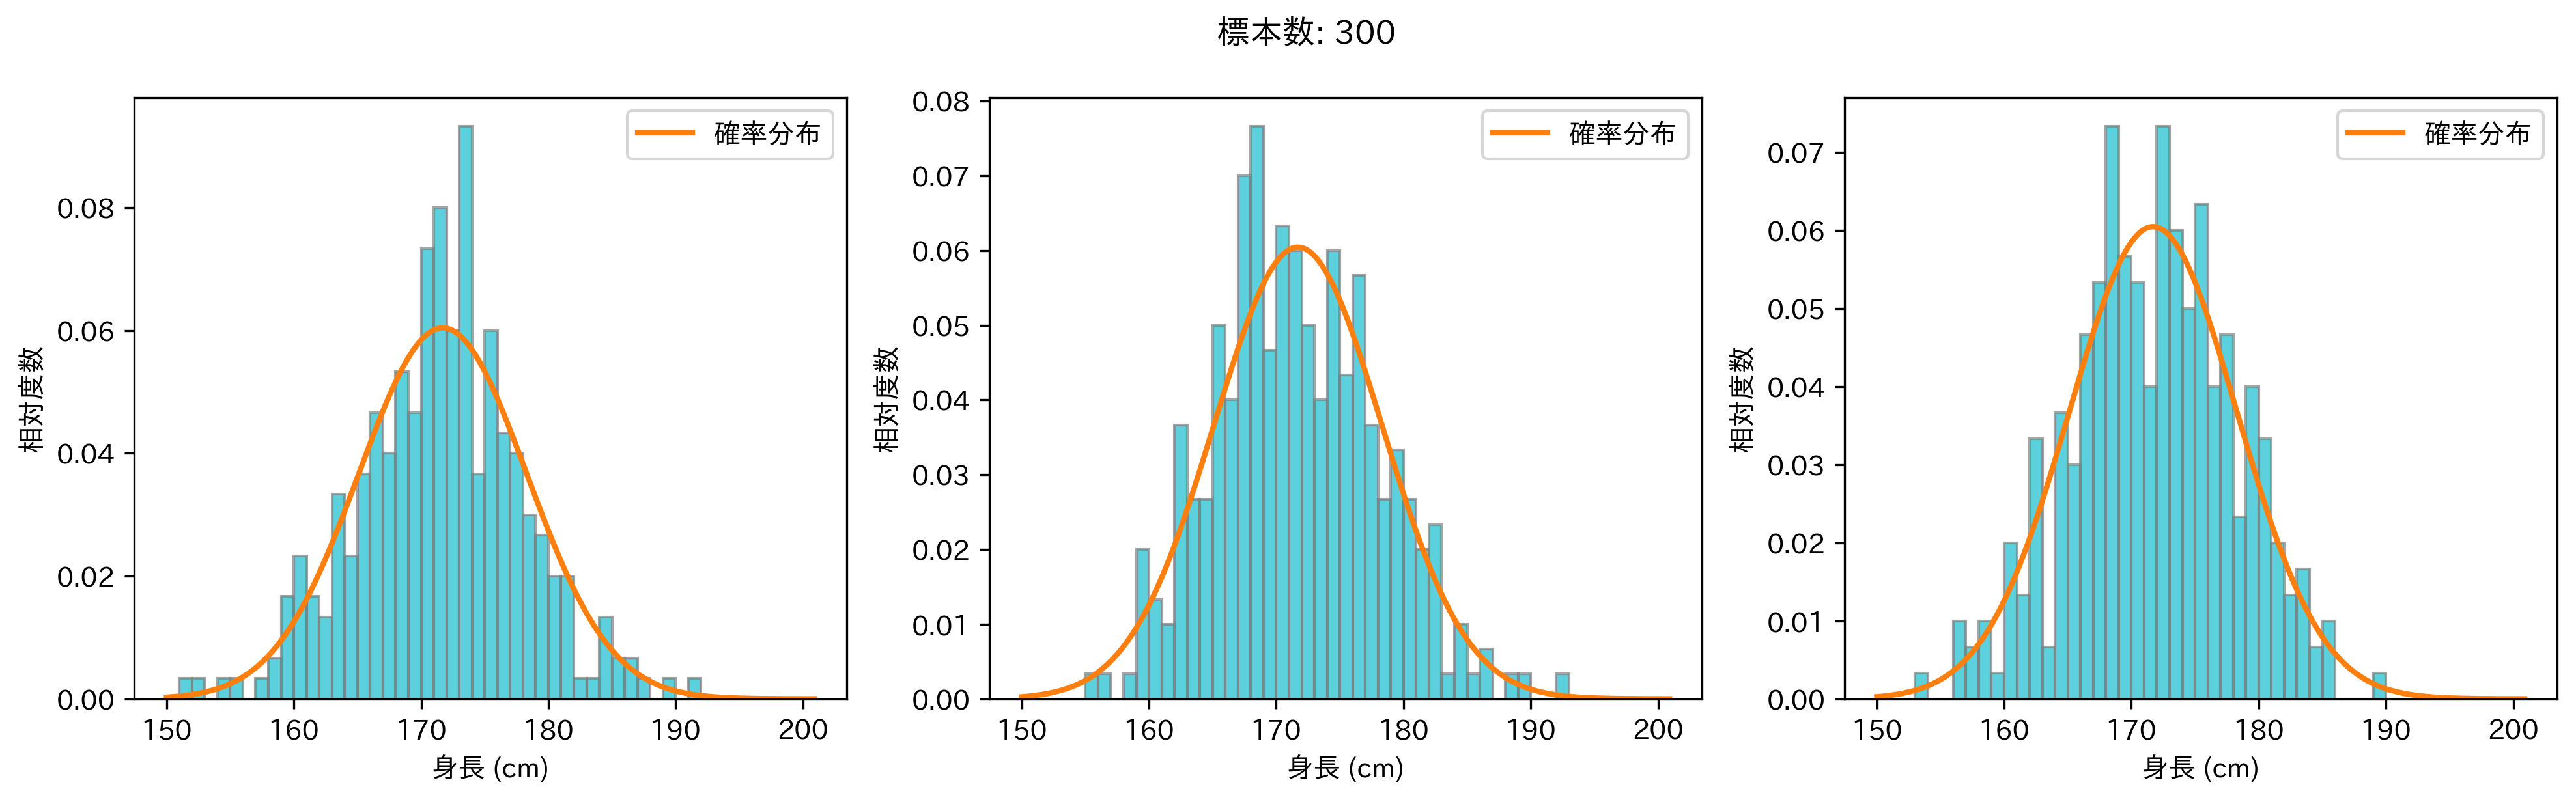
\includegraphics[width=0.95\linewidth]{./python/sampling-height_300.png}

しかし、この揺らぎは、標本数を大きくしていくと小さくなっていく。

すなわち、十分多くの標本を無作為抽出すれば、何度抽出を繰り返しても、得られる度数分布は一定の分布に近づく。

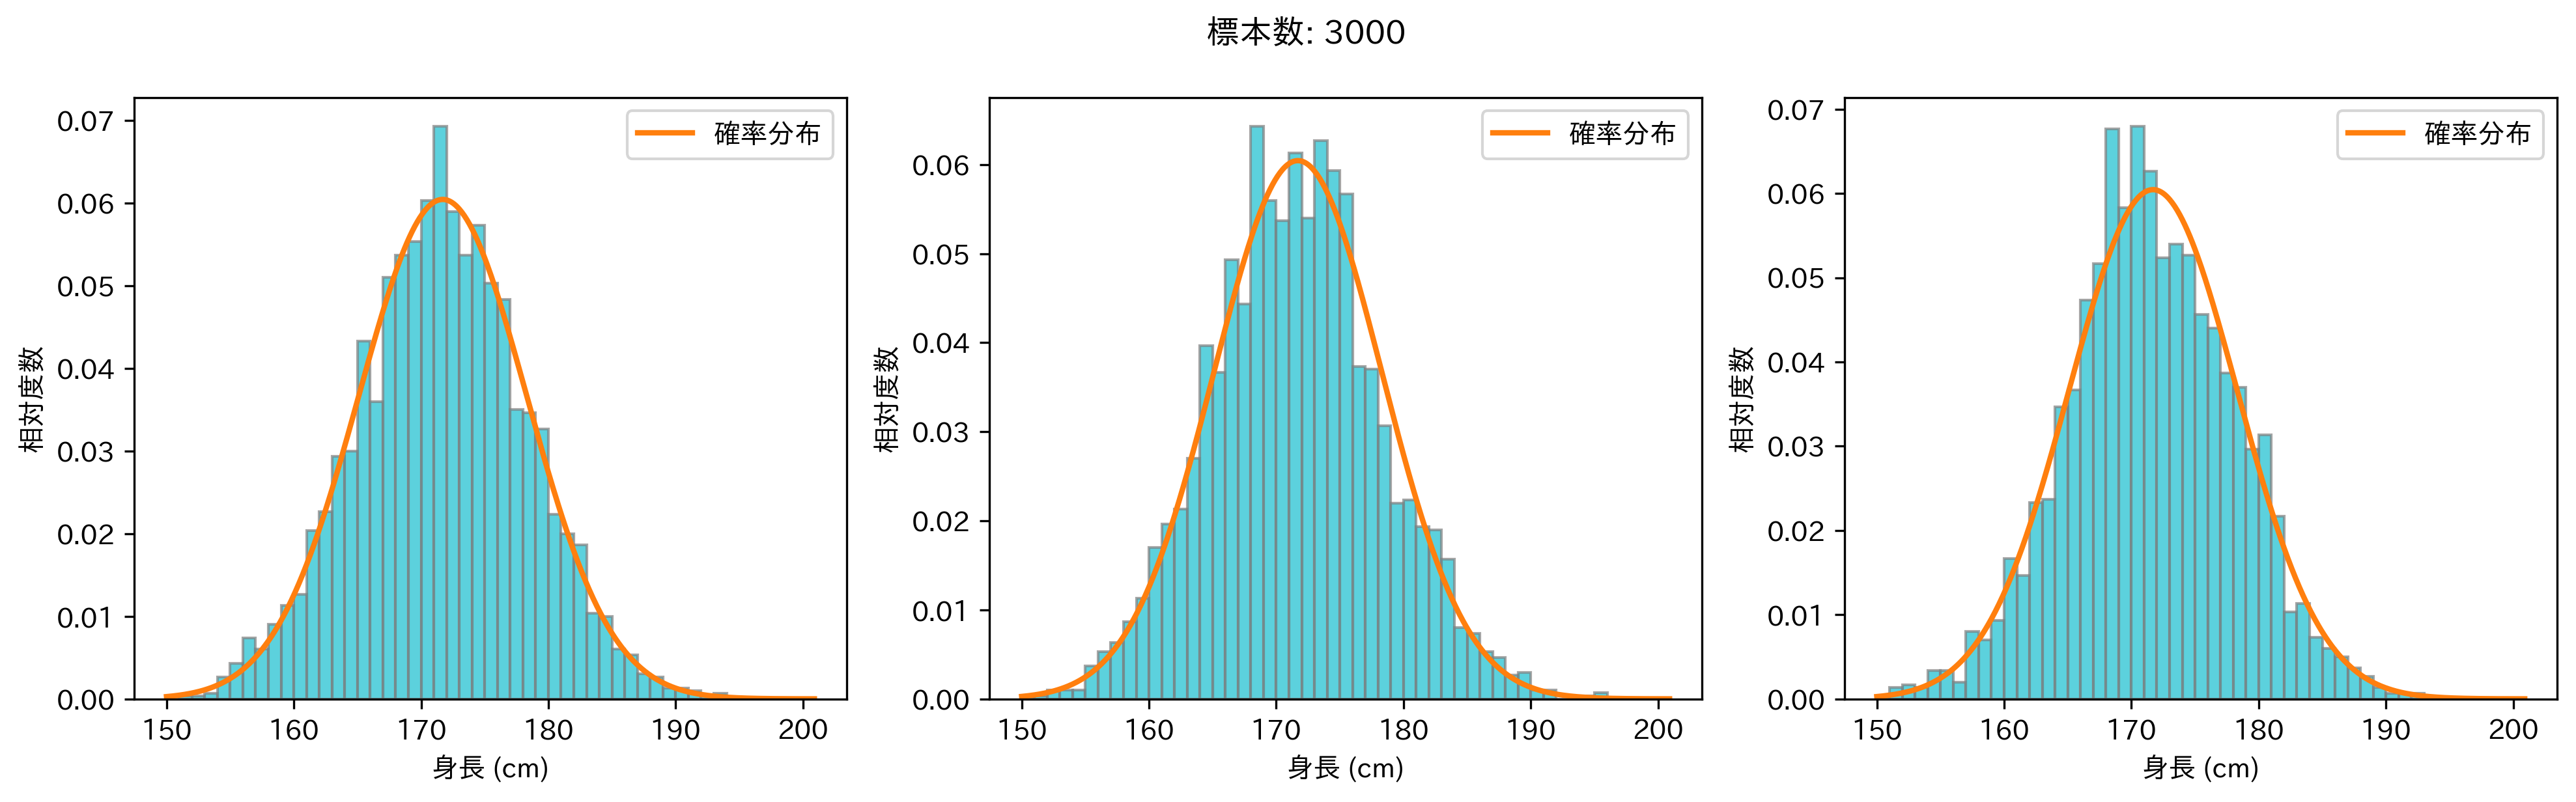
\includegraphics[width=0.95\linewidth]{./python/sampling-height_3000.png}

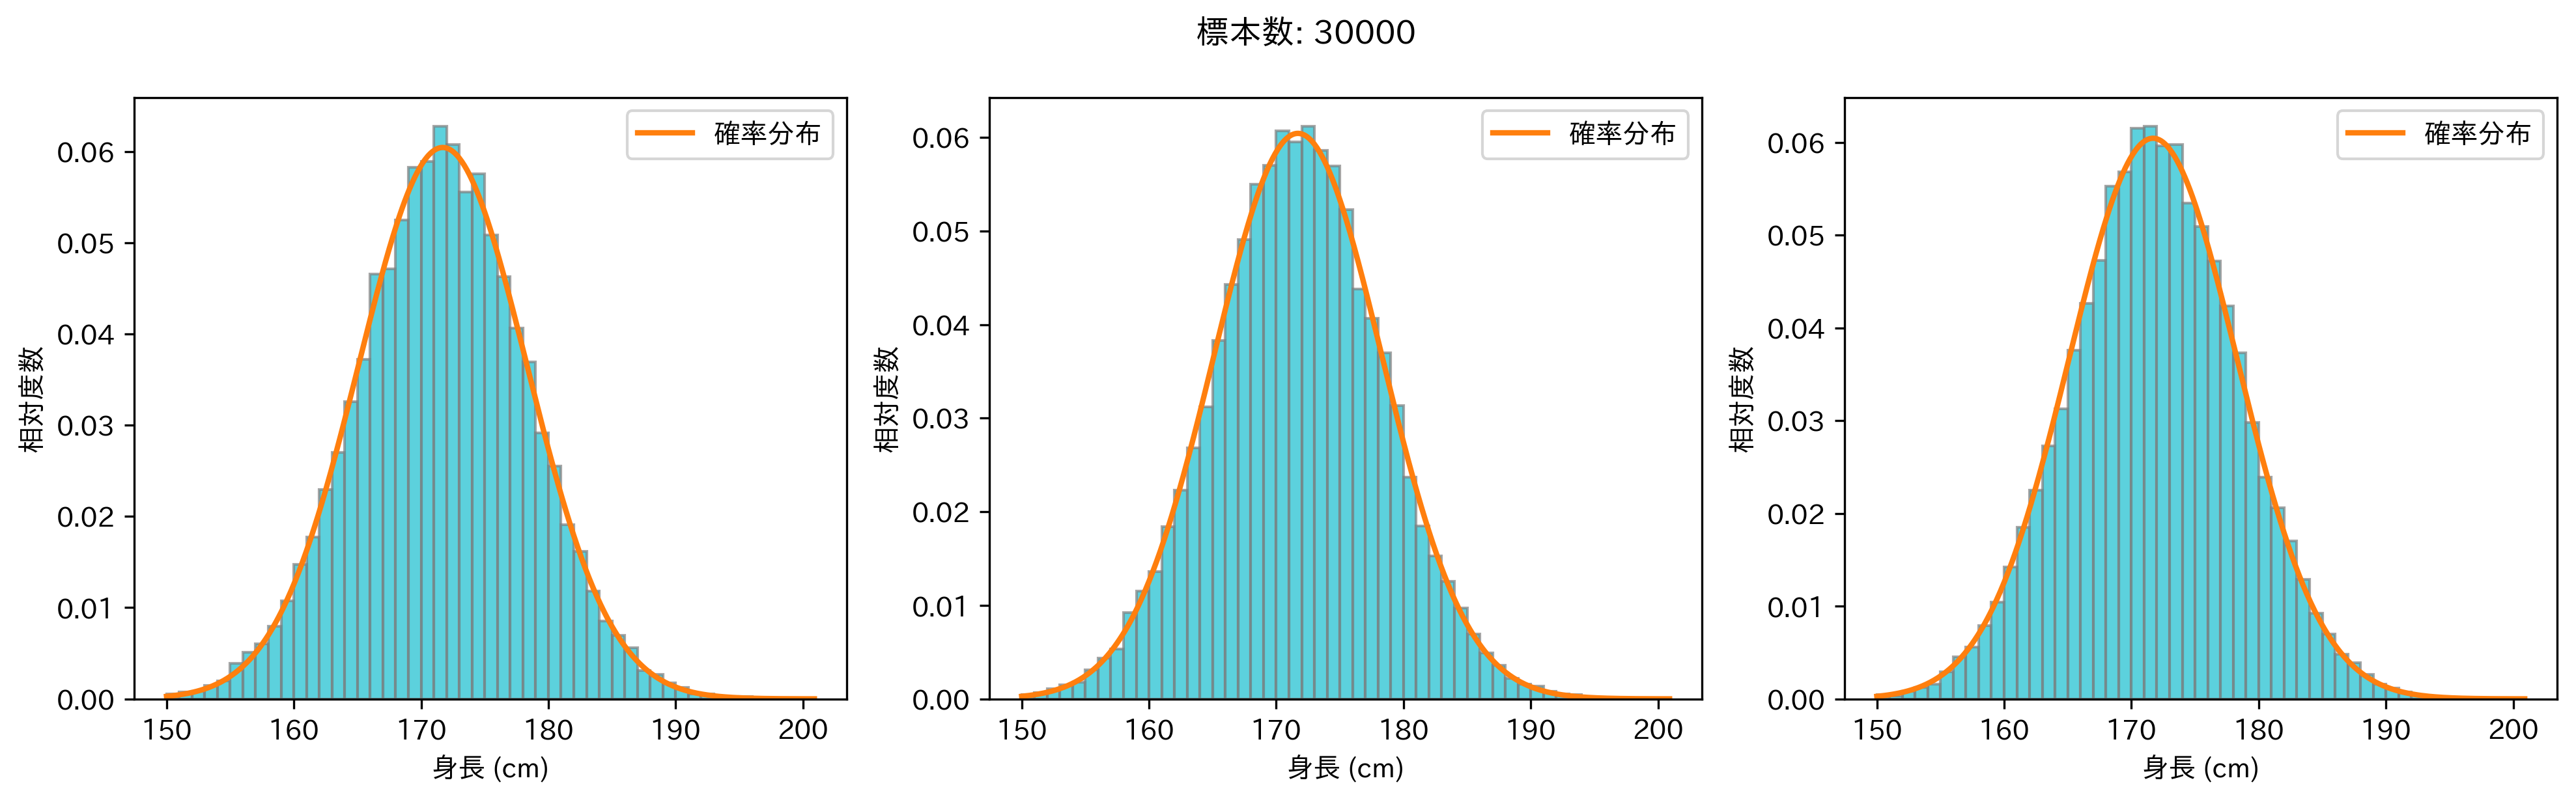
\includegraphics[width=0.95\linewidth]{./python/sampling-height_30000.png}

抽出する標本の数を大きくしていけばいくほど、抽出した「一部分」は「全体」に近くなっていくため、その度数分布は\keyword{母集団}の度数分布に近づいていくことになる。

\end{document}
